\section{MiSFP}\label{sec:method}
\subsection{Local Mixture Construction}
After inherited local contrastive training, client $i$ passes every eligible local training example through its encoder. Nonfinite rows are discarded and logged. For each class, seeded k-means++ and Lloyd updates fit centers; all features are then reassigned to those centers and streamed population moments are computed. A reservoir may fit centers when support exceeds 4096, but moments still use all eligible features. Components below minimum support are avoided by reducing $K$.

Fixed variants request $K\in\{1,2,4\}$. The adaptive variant forms a seeded fit/validation split within that class, evaluates $K=1,\ldots,K_{\max}$ using validation negative log likelihood per dimension plus $\lambda(K-1)$, retains $K=1$ unless the improvement exceeds threshold $\delta$, and refits on all class features. Insufficient validation/support falls back to $K=1$. This is a selection heuristic, not a consistent model-order theorem.

\begin{algorithm}[t]
\caption{Client packet construction}\label{alg:client}
\begin{algorithmic}[1]
\Require training features by class, mode, $K_{\max}$, support $s_{\min}$
\For{each represented class $c$}
 \State remove and count nonfinite rows
 \State select $K$ (fixed or held-out NLL threshold)
 \State fit seeded centers; reduce $K$ until supports are feasible
 \State assign all rows; compute $(n_{cr},\bm\mu_{cr},\bm v_{cr})$
\EndFor
\State compress under $B_{ce}$ if configured; serialize packet
\end{algorithmic}
\end{algorithm}

\subsection{Pooling and Budgeted Merging}
Received components retain their class but not a cross-source identity. For two same-class components with masses $a,b$, MiSFP uses
\begin{align}
m&=a+b,\qquad \bm\mu=(a\bm\mu_a+b\bm\mu_b)/m,\label{eq:poolmean}\\
\bm v&=\frac{a[\bm v_a+(\bm\mu_a-\bm\mu)^2]}{m}
+\frac{b[\bm v_b+(\bm\mu_b-\bm\mu)^2]}{m}.\label{eq:poolvar}
\end{align}
Squares are elementwise. The candidate pair score is
\begin{equation}\label{eq:mergecost}
\Delta(a,b)=\frac{ab}{a+b}\left(\|\bm\mu_a-\bm\mu_b\|_2^2+|\sqrt{\bm v_a}-\sqrt{\bm v_b}\|_2^2\right).
\end{equation}
The parenthesized term is $W_2^2$ between the two diagonal Gaussians. It is not the Wasserstein distance between the pre- and post-merge mixtures. Components are canonicalized for deterministic ties. MiSFP first merges to any per-class cap, then repeatedly chooses the feasible same-class pair with lowest $\Delta$ per byte saved. At least one component per represented class remains; a budget smaller than that packet is reported infeasible rather than dropping a class. Greedy merging is not globally optimal and can remove minority modes.

\subsection{Synthesis and Nonlinear Boundary Transformation}
For every synthetic feature, MiSFP first draws $r\sim\mathrm{Categorical}(\bm\pi_c)$ and then
\begin{equation}
 \tilde z=\bm\mu_{cr}+\sqrt{\max(\bm v_{cr},\epsilon_s)}\odot\xi,\quad\xi\sim\mathcal N(0,I).
\end{equation}
It never averages components before sampling. The inherited balanced class prior supplies $M_c$ samples per represented class. Variances remain unfloored in packets and pooling; floors are used only for NLL evaluation and sampling.

The edge trains $h_{\theta_e}$ with the inherited supervised-contrastive objective on synthetic inputs. Because nonlinear $h$ makes $h_\#Q_c$ generally non-Gaussian, input parameters cannot be relabeled as edge-output parameters. In default \emph{propagate} mode, the implementation draws the same Monte Carlo count from each incoming component, transforms those samples separately, and estimates an output mean and population variance. The output mass remains the component's original support; it is not the Monte Carlo count. Thus unequal mixture weights affect masses even though transformation estimates receive equal samples. In \emph{refit} mode, $M_c$ samples are drawn from the mixture, transformed, and reclustered; masses are assignment fractions times incoming support. Both are approximations.

The cloud concatenates compatible edge packets, optionally compresses them, samples a balanced synthetic dataset, and trains $g$ by cross entropy. Gradient paths end within each tier: no activation gradient is returned across a split. Same-tier model aggregation at slower intervals is inherited, not a prototype contribution.

\begin{algorithm}[t]
\caption{Edge receive--train--emit operation}\label{alg:edge}
\begin{algorithmic}[1]
\Require compatible client packets, caps/budgets, boundary mode
\State concatenate same-class components and compress edge input
\State sample component then feature; train $h$ locally on synthetic data
\If{propagate}
 \State transform a fixed MC count per input component; retain support mass
\Else
 \State sample per class, transform, and refit output mixture
\EndIf
\State compress output packet under cap and $B_{ec}$; serialize
\end{algorithmic}
\end{algorithm}

\begin{figure*}[t]
\centering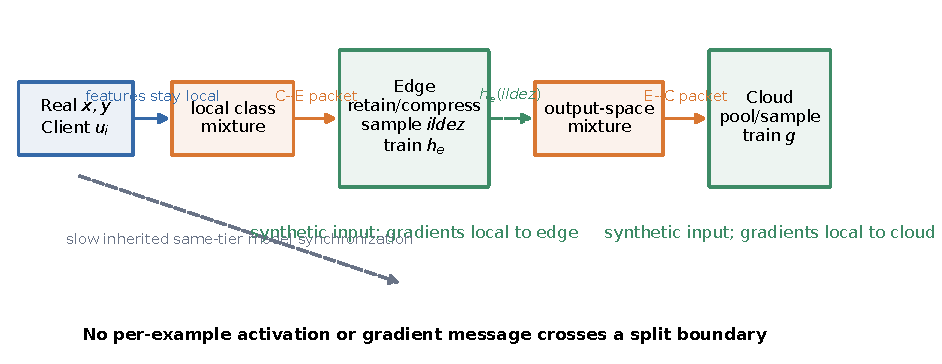
\includegraphics[width=.96\textwidth]{figures/misfp_architecture.pdf}
\caption{MiSFP client--edge--cloud execution. Solid blue arrows carry real inputs only within clients; orange arrows carry serialized class/component summaries; dashed green arrows denote locally generated features. Model gradients remain inside a tier. Slow same-tier model synchronization (gray) is inherited from H-SFP.}
\label{fig:architecture}
\end{figure*}

\begin{figure}[t]
\centering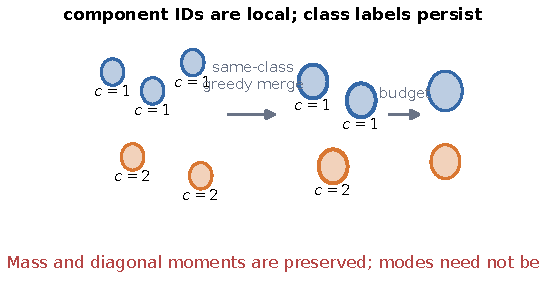
\includegraphics[width=\columnwidth]{figures/misfp_merging.pdf}
\caption{Class-preserving component retention and budgeted merging. Component identifiers are source-local; merging compares only components with the same class and preserves aggregate mass and diagonal moments, not density modes or decision boundaries.}
\label{fig:merging}
\end{figure}
